\section{Experimental Evaluation}
\label{MG:Sec:Experiment}

We evaluate the performance of \sysname using two large malware datasets, each with more than 10,000 samples, and present our experimental results in this section.

\subsection{Malware Datasets}
The first dataset, which we refer to as the \textit{MSKCFG} dataset, includes the CFGs derived from the malware files used in the 2015 Microsoft Malware Classification Challenge hosted by Kaggle~\cite{MsAcfgDataset}. The dataset contains samples that fall into nine families: \{Ramnit, Lollipop, Kelihos\_ver3, Vundo, Simda, Tracur, Kelihos\_ver1, Obfuscator.ACY, Gatak\}.
Figure~\ref{MG:Fig:MSKCFGLabelDist} presents the number of samples in each of these nine malware families in the dataset.
%The identification of benign code is not in the scope of the contest, and all the input files are supposed to be malicious.
In the competition, Kaggle provided 10,868 labeled malware samples as the training dataset, for each of which two files were given.
% Kaggle used another 10,873 malware samples, whose labels remained unknown to participants, to rank the submissions.
% We ignored 10 `empty'\footnote{A file is \textit{empty} if it contains only character `??', which means the data provider erased these byte information for certain reasons.} .byte files in training set and 13 empty ones in testing set respectively.
%Two files were given for each malware is represented as two files in the dataset.
The first file contains the raw binary content in a hexadecimal representation (referred as .byte file in the following discussion).
The second file is the corresponding assembly code of the binary code, which was generated with the IDA Pro tool~\cite{bib:idapro} (referred as .asm file in the following discussion).
The correctness of the .asm file is not guaranteed because PE headers were erased from the raw malware files for sterility before they were disassembled and sophisticated binary packing techniques may also prevent reverse engineering tools from disassembling the malware correctly~\cite{BinaryUnpacking}. 
In our experiments, only the .asm files were used for malware classification.
We generated a total number of 10,868 ACFGs from the training .asm files, which took approximately 17 hours to finish, or averagely 5.8 seconds per malware instance,
using a commodity desktop equipped with Intel Core i7-6850K CPU and 64 GB memory.
%These ACFGs are denoted as the \textit{MSKCFG} dataset hereafter.

Another dataset, which we refer to as \textit{YANCFG}, includes the CFGs of 16,351 binary executable files which were used in \cite{YanDataset}.
%The original dataset contains hexadecimal bytes from the original binary file and the features from both dynamic execution traces and PE headers.
%However, the dataset given to us are CFG format files.
Similar to the MSKCFG dataset, the PE headers were not available to us for malware classification from the second dataset. All the CFGs were labeled with a majority voting scheme based on the detection results of five major AV scanners returned by the VirusTotal online malware analysis service~\cite{VirusTotal}.
All the CFGs belong to 12 distinct malware families: \{Bagle, Benign, Bifrose, Hupigon, Koobface, Ldpinch, Lmir, Rbot, Sdbot, Swizzor, Vundo, Zbot, Zlob\}.
Figure~\ref{MG:Fig:YANCFGLabelDist} depicts the number of samples for each of these 12 families in the dataset.
These CFGs were further converted to their corresponding ACFGs by MAGIC within 6.8 hours using the same desktop machine as mentioned above.
%After the 6.8-hour CFG-to-ACFG conversion, we obtained 16,351 ACFGs.% further discarded 1,976 empty graphs.
%These ACFGs are stored together and referred as \textit{YANCFG} as a whole dataset.
%For clarity, we refer the second dataset as \textit{YANCFG}.
%We plan to make the resultant ACFGs on both public and private datasets available to the research community alongside with the system implementation of \sysname.


We did not merge two malware datasets in our experiments due to the following reasons.
Firstly, the YANCFG dataset carries pre-processed CFGs,
while we developed our own parser to extract CFGs from the malware assembly code in the Microsoft dataset (see Section~\ref{MG:SubSec:BuildCfg}).
% The differences in the methods used to extract CFGs from the two datasets may lead to inconsistent CFG representations for model training.
The CFG extracted from the MSKCFG dataset by our own parser has different low-level feature representation from that of the CFGs pre-given in YANCFG;
so they cannot be applied to one model.
Secondly, testing MAGIC on datasets collected from independent sources also allows us to gain insights into its generality when applied in different operational environments.

\begin{table}[ht]
    \begin{center}
        \begin{tabular}{l|r}
            \hline
            Hyperparameter & Choice or Value Range \\
            \hline
            \hline
            Pooling Type & [Adaptive Pooling, Sort Pooling] \\
            \hline
            Pooling Ratio & [0.2, 0.64] \\
            \hline
            Graph Convolution Size & [(32, 32, 32, 1)\tablefootnote{Only for sort pooling}, (32, 32, 32, 32), (128, 64, 32, 32)] \\
            \hline
            Remaining Layer\tablefootnote{Applicable only when set \textit{pooling type} to sort} & [1D Convolution Layer, WeightVertices Layer] \\
            \hline
            2D Convolution Channels\tablefootnote{Applicable only when set \textit{pooling type} to adaptive pooling} & [16, 32] \\
            \hline
            1D Convolution Channel Pairs\tablefootnote{Applicable only when set \textit{pooling type} to sort pooling and \textit{remaining layer} to 1D convolution} & [(16, 32)] \\
            \hline
            1D Convolution Kernel Size\tablefootnote{Applicable only when set \textit{pooling type} to sort pooling and \textit{remaining layer} to 1D convolution} & [5, 7] \\
            \hline
            Dropout Rate & [0.1, 0.5] \\
            \hline
            Batch Size & [10, 40] \\
            \hline
            Weight L2 Regularization Factor & [0.0001, 0.0005] \\
            \hline
        \end{tabular}
        \caption{Hyperparameters and Search Ranges during Tuning}
        \label{MG:Tab:Hyperparameters}
    \end{center}
\end{table}

\begin{table}
    \begin{center}
        \begin{tabular}{l|r|r}
            \hline
            Hyperparameter & For MSKCFG & For YANCFG \\
            \hline
            \hline
            Pooling Type & Adaptive Pooling &  Adaptive Pooling\\
            \hline
            Pooling Ratio & 0.64 & 0.2 \\
            \hline
            Graph Convolution Size & (128, 64, 32, 32) & (32, 32, 32, 32)\\
            \hline
            Remaining Layer & Not Applicable &  Not Applicable \\
            \hline
            2D Convolution Channels & 16 & 16 \\
            \hline
            1D Convolution Channel Pairs & Not Applicable & Not Applicable \\
            \hline
            1D Convolution Kernel Size & Not Applicable & Not Applicable\\
            \hline
            Dropout Rate & 0.1 & 0.5 \\
            \hline
            Batch Size & 10 & 40\\
            \hline
            Weight L2 Regularization Factor & 0.0001 & 0.0005\\
            \hline
        \end{tabular}
        \caption{Optimal Hyperparameters for Both MSKCFG and YANCFG Datasets}
        \label{MG:Tab:BestHyperparameters}
    \end{center}
\end{table}

\subsection{Model Training and Evaluation}
As the malware families are different in the two datasets, we need to create two different \sysname instances to classify their malware samples separately. However, MAGIC uses the same way to train DGCNN and tune its hyperparameters for both datasets.
The first step is hyperparameter tuning.
Table~\ref{MG:Tab:Hyperparameters} lists the hyperparameters used in both the deep neural network itself (e.g., the sizes of the graph convolution layers) and the algorithm for training the model (e.g., batch size and learning rate).
To determine the optimal values of these hyperparameters,
we exhaustively search all 208 hyperparameter settings defined by the value ranges listed in Table~\ref{MG:Tab:Hyperparameters}.
In particular, 64 DGCNN models use adaptive pooling, 96 DGCNN models use the sort pooling and Conv1D layer, and 48 DGCNN models use the sort pooling and WeightVertices layer.
We apply the five-fold cross-validation technique to evaluate the performance of a model under a specific hyperparameter setting.
To conduct five-fold cross validation, the dataset is splitted into five equal-size subsets.
In each fold of the cross validation, four subsets (80\%) of the data are used for training a brand new model initialized randomly,
and the rest subset (20\% of the data), different in each fold, is used to evaluate the resultant model.
In this way, the training process never sees the testing samples used for performance evaluation.
We train each model with 100 epochs and record the negative log-likelihood validation loss after every epoch.
%The average loss score over the five cross-validation runs is reported.

The validation loss collected after each epoch is used to find the hyperparameters that can mitigate the overfitting issue. Once the validation loss increases for two continuous epochs,
we decrease the learning rate by a factor of ten to prevent the model from overfitting the training dataset.
For a particular model, when all five training-validation folds are finished, we compute each epoch's validation loss by averaging the five validation losses over the five folds.
The minimum validation loss over the 100 epochs is treated as the score of this model and is further used as the criterion for comparing with different hyperparameter settings.
In other words, after the five-fold cross-validation for all the 208 model training instances, we choose the best model with the minimum average validation loss.
%To compare our best model's performance to previous works, 
Besides the average validation negative log-likelihood loss,
we also measure its precision, recall, and F1 score averaged over the five validation sets (together referred to as the \emph{cross-validation scores}), and then compare the best model's performance against those of previous works.
We used four GeForce GTX 1080 Ti graphic cards to train and run the 208 variants of DGCNN.
Training a particular model is always done on a single GPU,
but the evaluation procedure actually takes up all the four GPUs because our \sysname implementation supports parallel model training on multiple GPUs.
Table~\ref{MG:Tab:BestHyperparameters} describe the best models chosen by MAGIC for the MSKCFG and YANCFG datasets, respectively.
% Confusion matrix for a random validation set is also included.
%Their cross-validation scores are reported in the following two sub-sections for both MSKCFG and YANCFG dataset respectively.
In the following, we report the cross-validation scores for the two datasets.

\begin{figure}
    \centerline{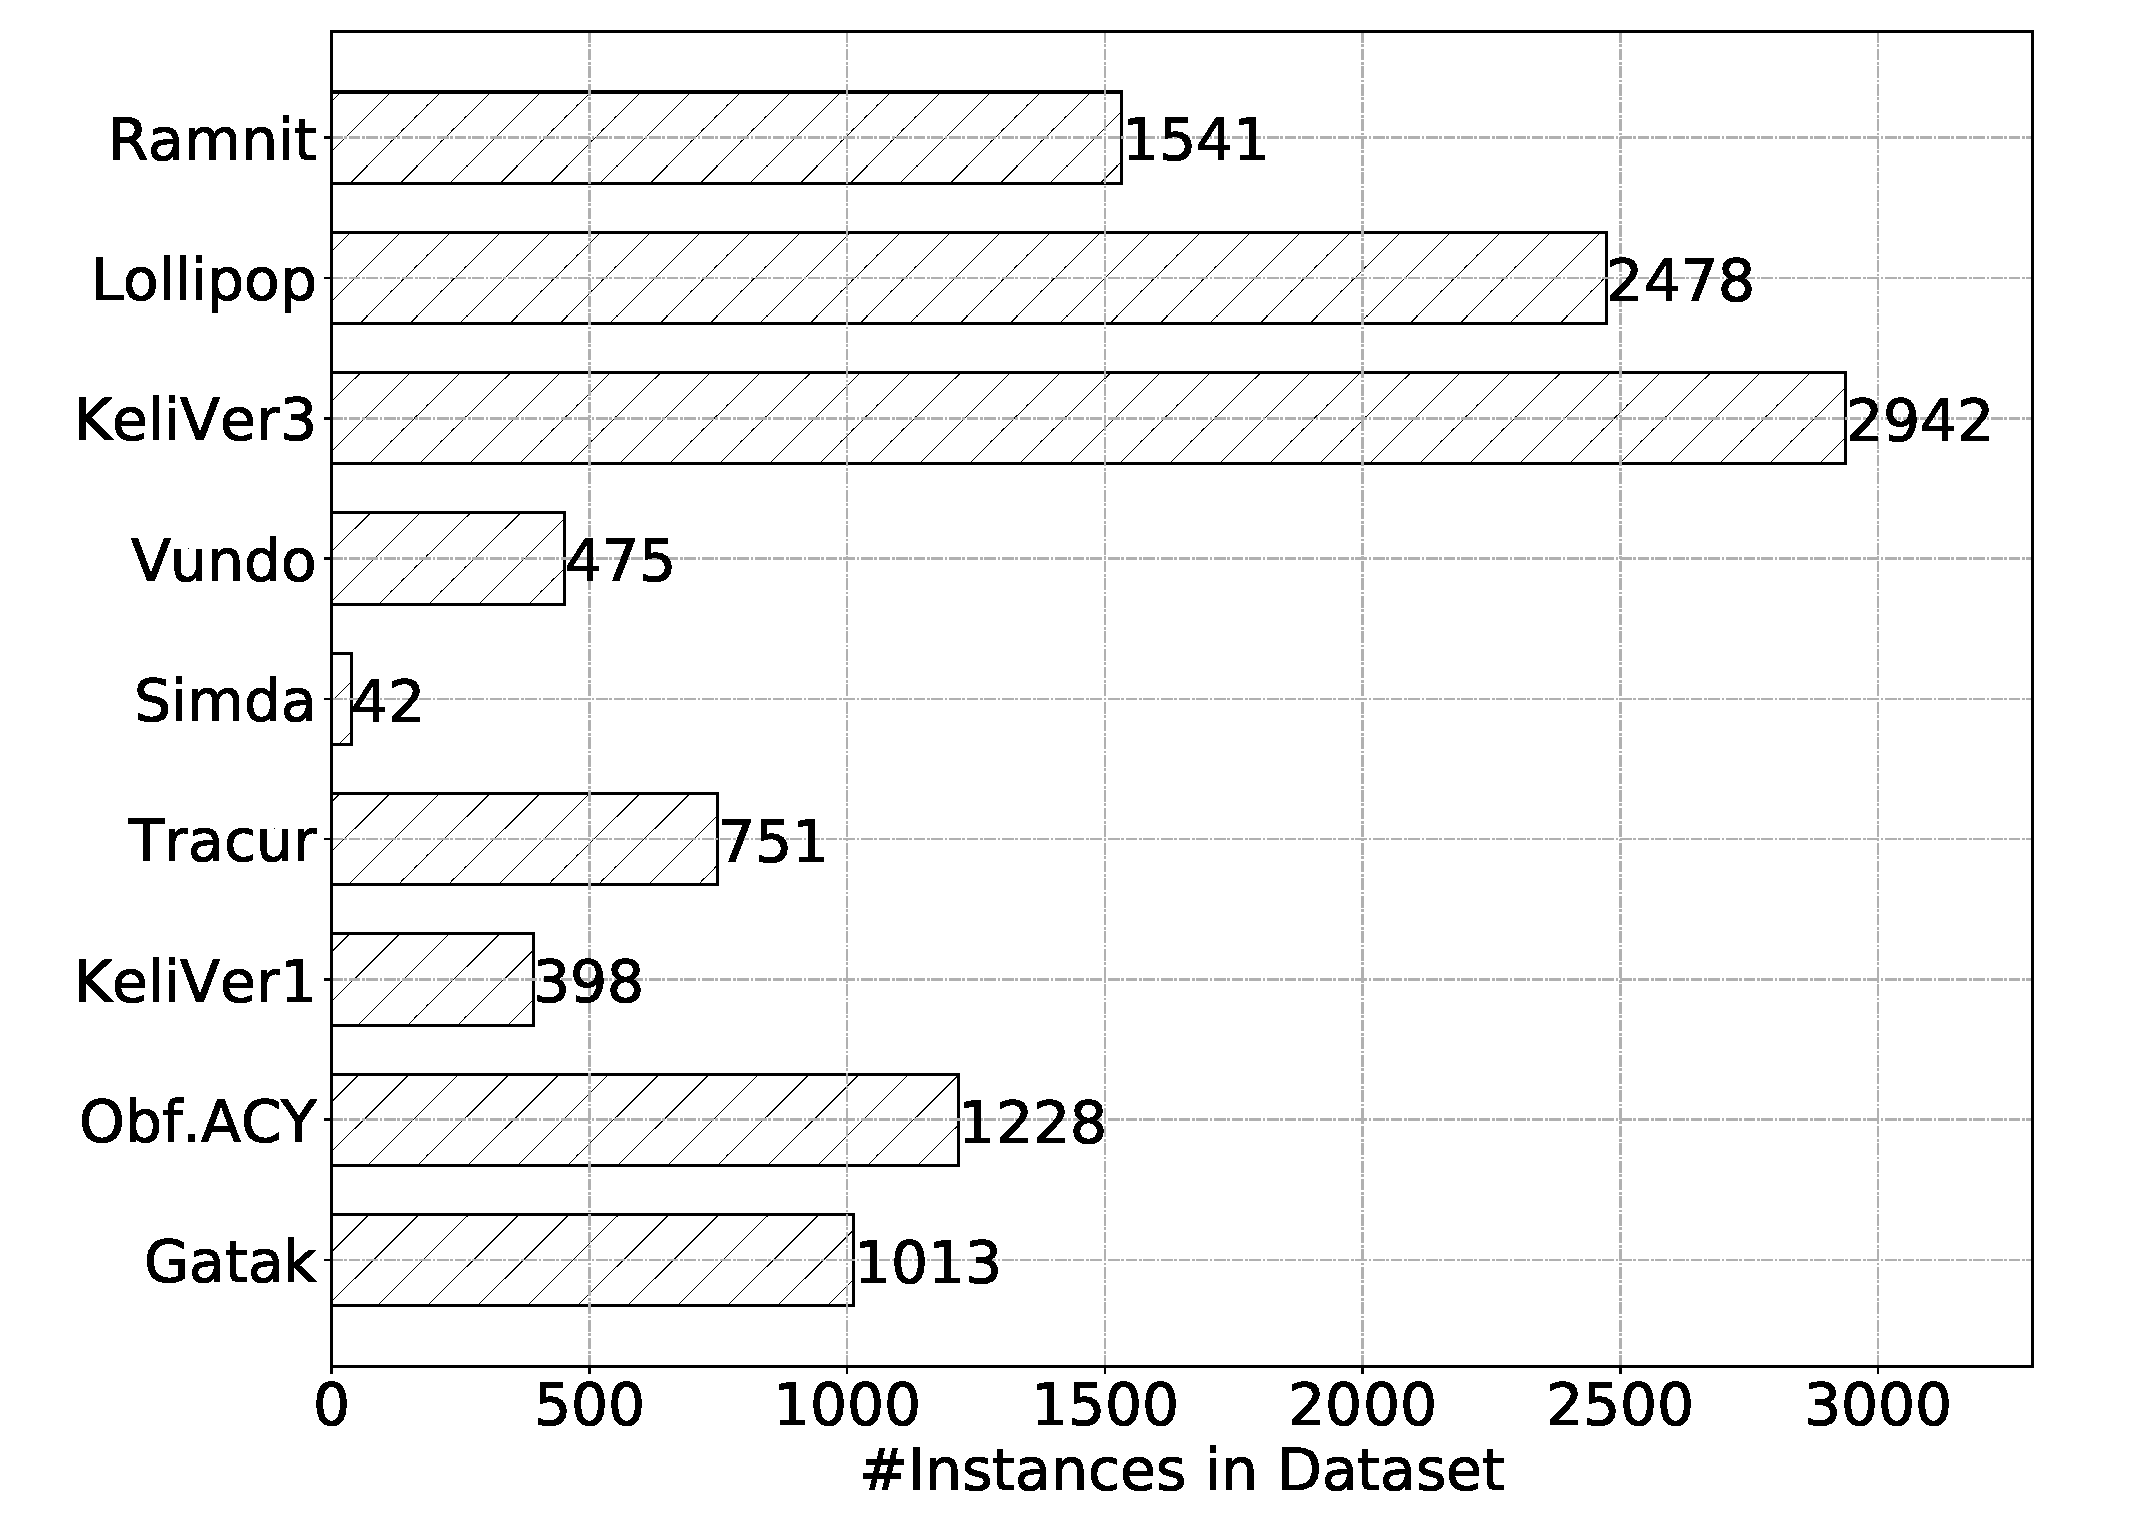
\includegraphics[width=0.90\textwidth]{Magic/figures/MsAcfgLabelDist.eps}}
    \caption{Malware Family Distribution in MSKCFG Dataset.}
    \label{MG:Fig:MSKCFGLabelDist}
\end{figure}

\begin{figure}
    \centerline{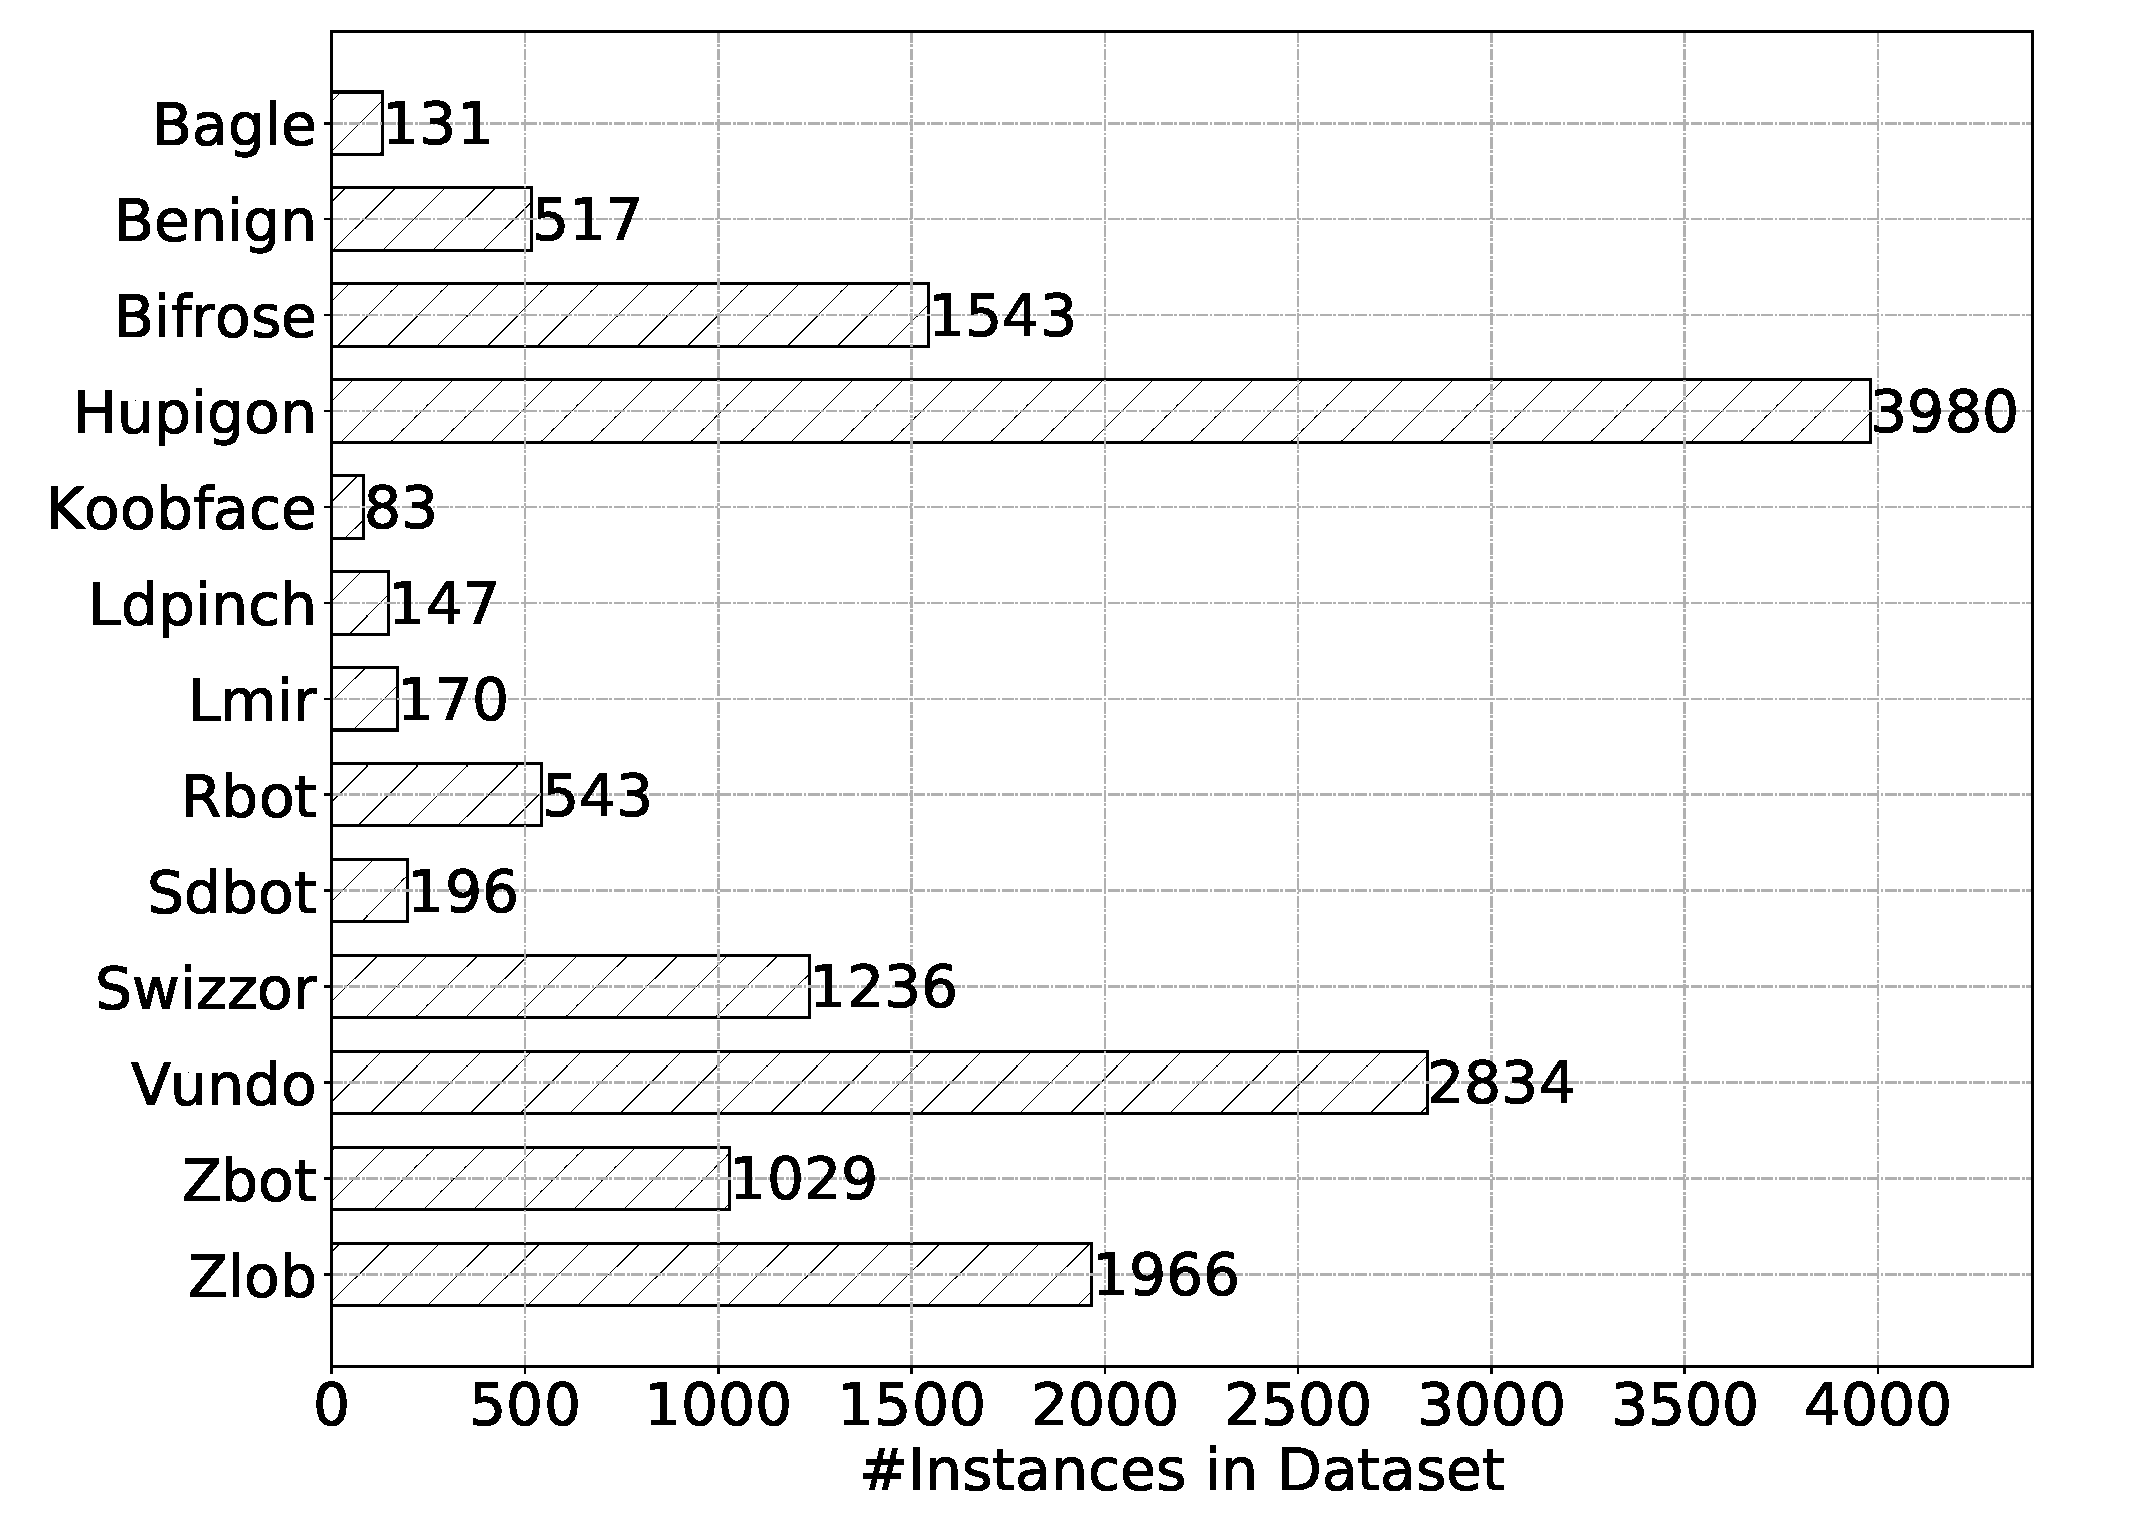
\includegraphics[width=0.90\textwidth]{Magic/figures/YanAcfgLabelDist.eps}}
    \caption{Malware Family Distribution in YANCFG Dataset.}
    \label{MG:Fig:YANCFGLabelDist}
\end{figure}

\subsection{Results on the MSKCFG Dataset}
The best cross-validation scores (precision, recall and F1) for the MSKCFG dataset are shown in Figure~\ref{MG:Fig:MSKCFGScores}, and the exact score values are listed in Table~\ref{MG:Tab:MSKCFGScores}.
The standard variances are not listed because the scores' variations among five different cross-validation folds are negligible ($<0.004$).
% Table~\ref{tab:MSKCFGConfusionMatrix} details the corresponding confusion table.
For all nine malware families, our best model has achieved good validation scores with precisions higher than 0.96, recalls higher than 0.96, and F1-scores higher than 0.97.

\begin{figure}
    \centerline{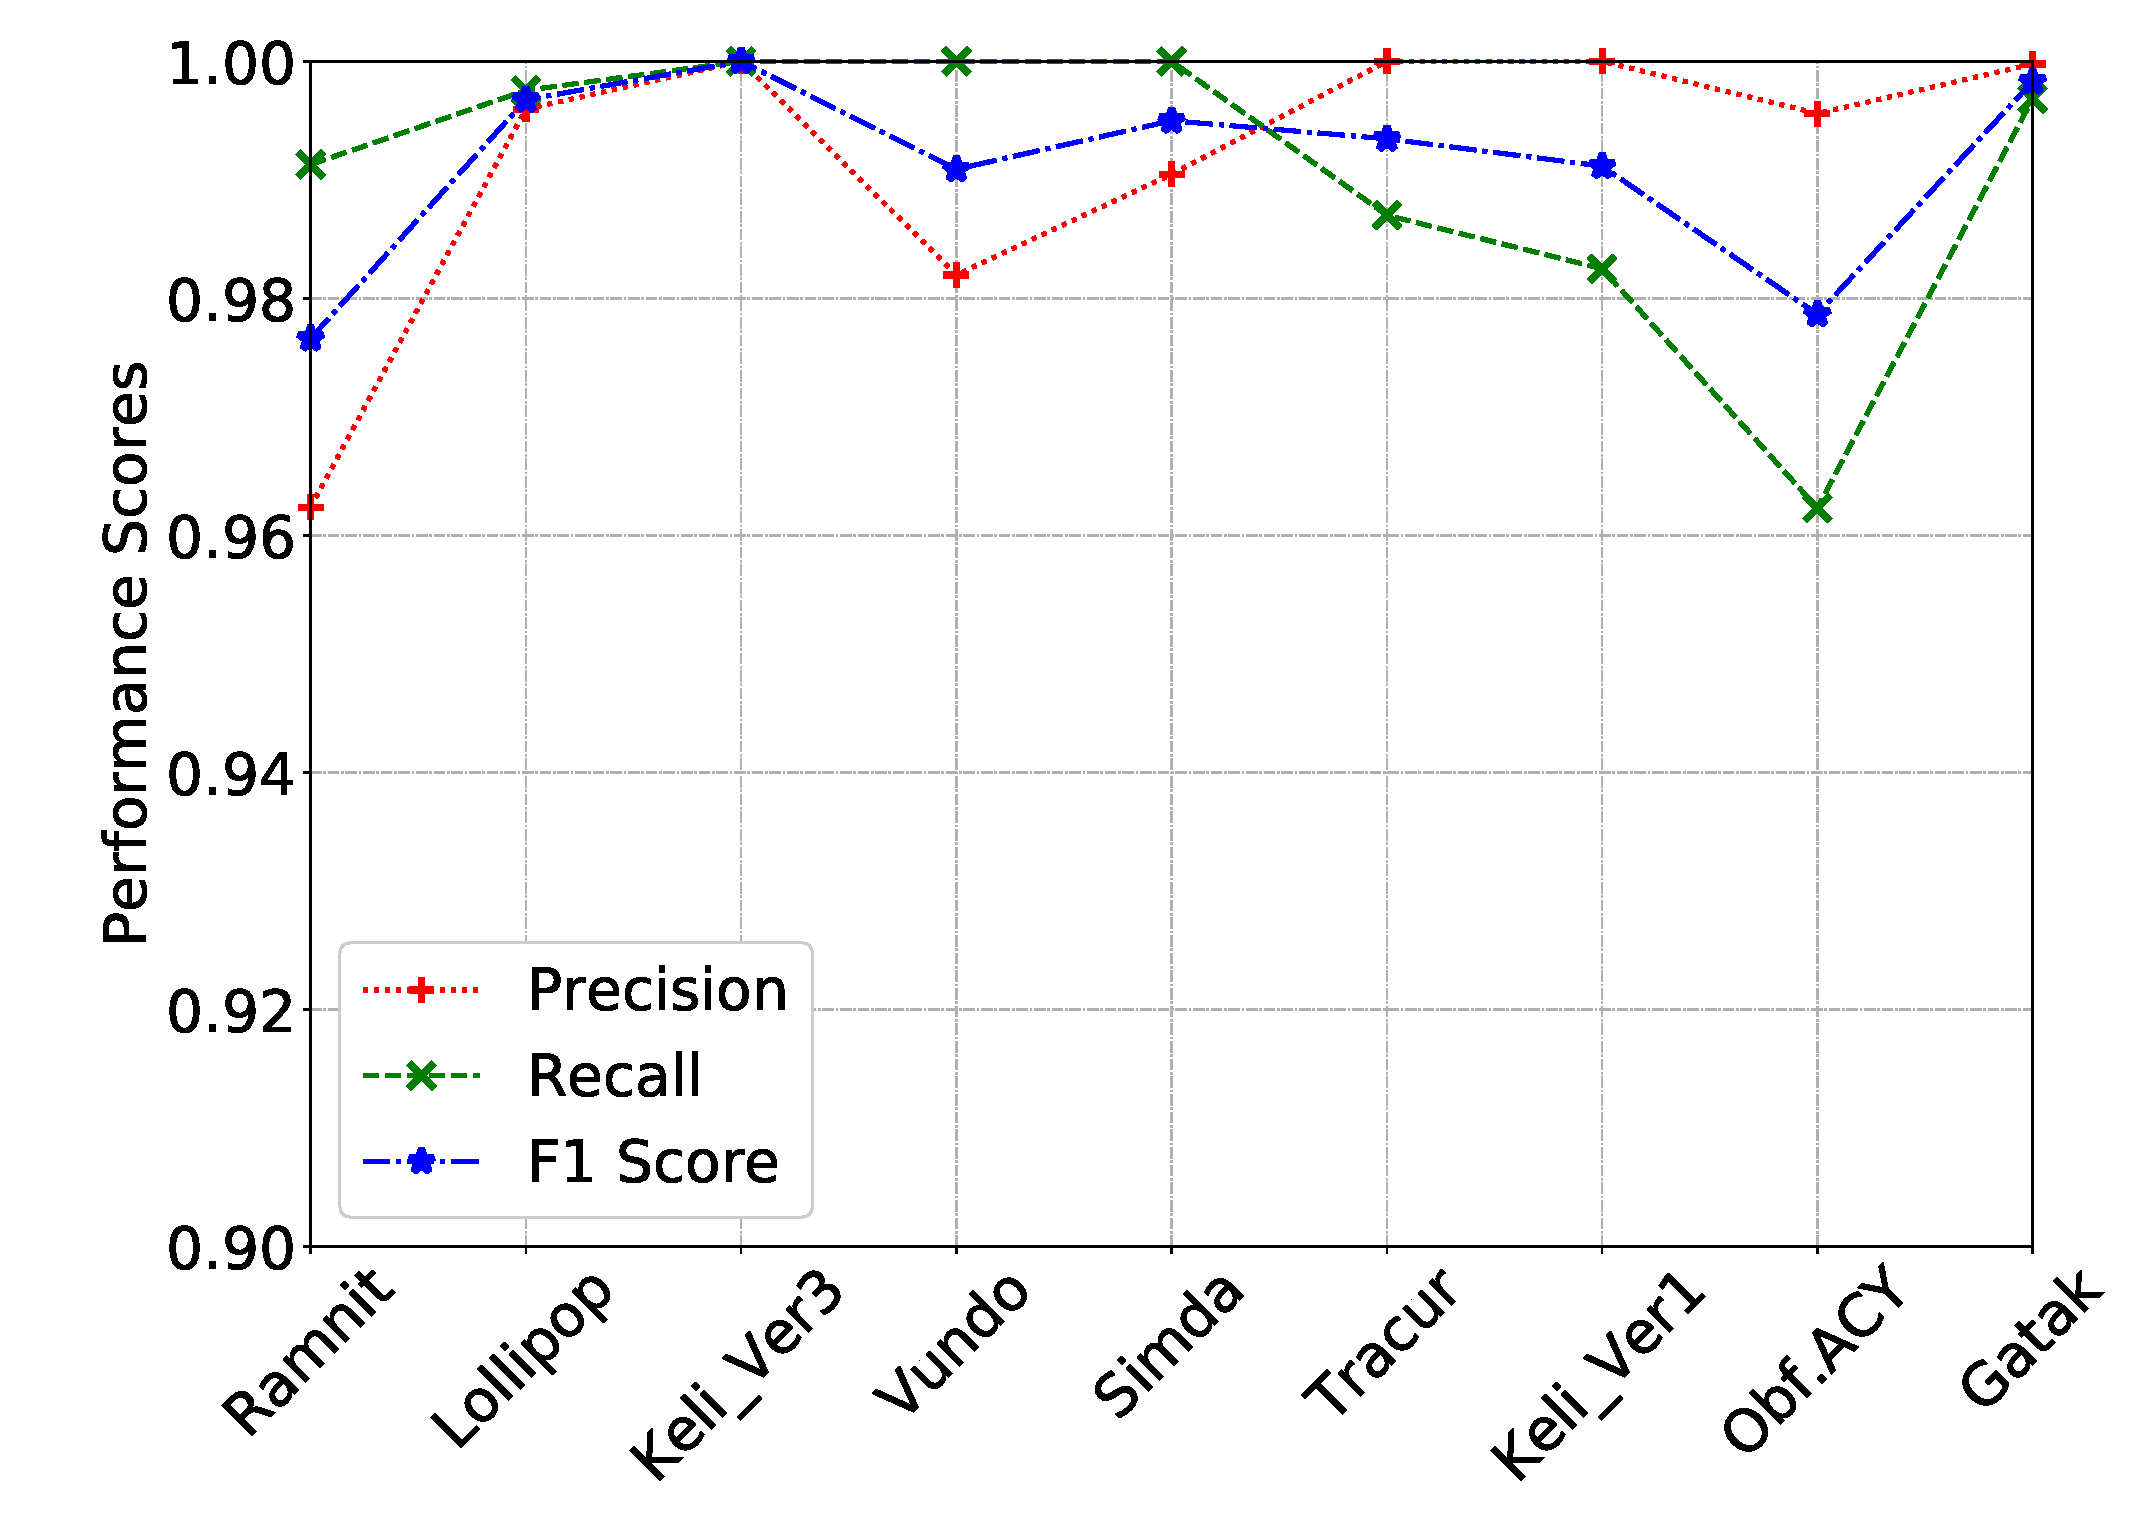
\includegraphics[width=0.90\textwidth]{Magic/figures/MsAcfgScores.eps}}
    \caption{Cross-Validation Scores of \sysname on the MSKCFG Dataset.}
    \label{MG:Fig:MSKCFGScores}
\end{figure}

\begin{table}
    \caption{Performances of \sysname on the MSKCFG Dataset.}
    \begin{center}
        \begin{tabular}{l|rrr}
            \hline
            Family       &  Precision &    Recall &        F1 \\
            \hline
            \hline
            Ramnit       &   0.962378 &  0.991289 &  0.976615 \\
            Lollipop       &   0.995960 &  0.997550 &  0.996754 \\
            Kelihos\_Ver3  &   1.000000 &  1.000000 &  1.000000 \\
            Vundo       &   0.981975 &  1.000000 &  0.990895 \\
            Simda       &   0.990476 &  1.000000 &  0.994987 \\
            Tracur       &   1.000000 &  0.987013 &  0.993463 \\
            Kelihos\_Ver1  &   1.000000 &  0.982493 &  0.991156 \\
            Obfuscator.ACY  &   0.995593 &  0.962293 &  0.978655 \\
            Gatak       &   0.999775 &  0.996841 &  0.998304 \\
            \hline
        \end{tabular}
    \end{center}
    \label{MG:Tab:MSKCFGScores}
\end{table}

Since Microsoft released the competition dataset in 2015, many researchers have used the dataset (completely or partially) to evaluate their techniques for malware detection and classification~\cite{NovelFeatureFusion, EnsembleDNN, AutoEncoderMicrosoft, FunctionCallGraph, StaticFeatures, PolySeqCls, AutoEncoderFeatureLearn, YuxinMalwareDnn}.
We surveyed the works mentioned above and found that three of them cannot be directly compared with our results because they were using different metrics.
%and found that unfortunately every work either performed the evaluation in a unique way or gave their evaluation results using divided metrics due to varying reasons, making three works not directly comparable to ours. 
The works in \cite{EnsembleDNN} and \cite{YuxinMalwareDnn} used the Microsoft dataset in the context of \emph{malware detection}, where all the samples contained within it were treated as malicious, and then they were merged with a number of benign programs to construct a new dataset for malware detection.
As a result, their methods and performance metrics (two-class AUC, F1 score or accuracy) are not directly comparable to the approaches aimed at classifying malware samples into the corresponding families (e.g.,~\cite{NovelFeatureFusion, AutoEncoderMicrosoft, FunctionCallGraph, StaticFeatures, PolySeqCls, AutoEncoderFeatureLearn}), this work included. %, where models should predict the malware family that a sample belongs to.
Note that without loss of generality, benign software can be treated as a special family.
The work in~\cite{AutoEncoderMicrosoft} did not adopt the cross-validation methodology. Instead, the authors manually split the training dataset into 75\% training data and 25\% holdout testing data, and reported the mean square error, accuracy and confusion matrix over both training and testing data.
The holdout set is not the test set provided by Microsoft. 
Therefore, we did not compare our work with the evaluation results reported in \cite{EnsembleDNN}, \cite{YuxinMalwareDnn} and \cite{AutoEncoderMicrosoft}.

Among the other five papers of malware classification, both \cite{FunctionCallGraph} and \cite{StaticFeatures} conducted the ten-fold cross validation over the Microsoft dataset, but only reported the overall accuracy.
\cite{PolySeqCls} also performed a ten-fold cross validation but reported both the overall accuracy and logarithmic loss.
Both \cite{NovelFeatureFusion} and \cite{AutoEncoderFeatureLearn} performed a five-fold cross validation and reported both the overall accuracy and logarithmic loss.
Since the Microsoft dataset is not balanced across malware families, we compare \sysname with the five previous works that reported not only the overall accuracy but also the mean logarithmic loss, and the results are shown in Table~\ref{MG:Tab:CompareMicrosoftCv}.

The methods listed in Table~\ref{MG:Tab:CompareMicrosoftCv} can be classified into either ensemble-learning or single-model based approaches.
\cite{NovelFeatureFusion} extracts more than 1800 features and uses gradient boosting based classifier, and it achieves the best log-loss (0.0197) and accuracy (99.42\%) using the XGBoost classifier. 
\cite{FunctionCallGraph} achieves the second best accuracy (99.3\%) by ensembling multiple random forest methods, which already ensembles multiple decision trees.
The DGCNN-based technique used by MAGIC achieves highly competitive results.
In fact, the logarithmic loss (0.0543) is the second best; the accuracy (99.25\%) is the third best, only 0.005 less than the second best one (99.3\% reported by \cite{FunctionCallGraph}).
\cite{AutoEncoderFeatureLearn} adopts a deep-learning based hybrid approach.
It relies on a single deep autoencoder to perform automatic feature learning, and then uses gradient-boosting based classifier to make the prediction.
As an alternative work that also applies deep neural network, our DGCNN-based approach outperforms the work in~\cite{AutoEncoderFeatureLearn} by 27.40\% in terms of logarithmic loss and 1.5\% in terms of classification accuracy.
%regarding log-loss (27.40\% improvement) and accuracy (1.5\% improvement).

\begin{table*}
    \caption{Cross Validation Metric Comparison on the Microsoft Dataset.}
    \begin{center}
        \begin{tabular}{l|rr}
            \hline
            Approach Brief Description                                           & Mean Logarithmic Loss     & Accuracy \\
            \hline
            \hline
            \sysname                                                                &               0.0543      &   99.25 \\
            XGBoost with Heavy Feature Engineering\cite{NovelFeatureFusion}         &               0.0197      &   99.42 \\
            Deep Autoencoder based XGBoost\cite{AutoEncoderFeatureLearn}            &               0.0748      &   98.20 \\
            Strand Gene Sequence Classifier\cite{PolySeqCls}                        &               0.2228      &   97.41 \\
            Ensemble Multiple Random Forest Classifiers\cite{FunctionCallGraph}     &       Not Reported        &   99.30 \\
            Random Forest with Feature Engineering\cite{StaticFeatures}             &       Not Reported        &   99.21 \\
            \hline
        \end{tabular}
    \end{center}
    \label{MG:Tab:CompareMicrosoftCv}
\end{table*}


% \begin{table*}
% \centering
% \caption{Confusion Matrix on the MSKCFG Dataset}
% \begin{tabular}{l|rrrrrrrrr}
%   Family       &  Ramnit &  Lollipop & Kelihos\_Ver3 &  Vundo &  Simda &  Tracur & Kelihos\_Ver1 & Obfuscator.ACY &  Gatak \\
% \hline
% \hline
%    Ramnit       &     321 &         2 &             0 &      0 &      0 &       2 &             0 &              3 &      0 \\
%  Lollipop       &       4 &       443 &             0 &      0 &      0 &       0 &             0 &              0 &      0 \\
% Kelihos\_Ver3   &       0 &         0 &           586 &      0 &      0 &       0 &             0 &              0 &      0 \\
%     Vundo       &       0 &         0 &             0 &     88 &      0 &       0 &             0 &              0 &      0 \\
%     Simda       &       0 &         1 &             0 &      0 &      8 &       0 &             0 &              0 &      0 \\
%    Tracur       &       1 &         1 &             0 &      0 &      0 &     174 &             0 &              0 &      0 \\
% Kelihos\_Ver1   &       0 &         0 &             0 &      3 &      0 &       0 &            65 &              0 &      0 \\
% Obfuscator.ACY  &       9 &         1 &             0 &      0 &      0 &       0 &             0 &            235 &      0 \\
%     Gatak       &       0 &         0 &             0 &      1 &      0 &       0 &             0 &              0 &    210 \\
% \end{tabular}
% \label{MG:Tab:MSKCFGConfusionMatrix}
% \end{table*}


\subsection{Results on the YANCFG Dataset}
\sysname's best cross validation scores on the YANCFG dataset are depicted in Figure~\ref{MG:Fig:YANCFGScores} and the exact values of these scores are listed in Table~\ref{MG:Tab:YANCFGScores}.
% Table~\ref{tab:YANCFGScores} is the corresponding confusion table on the 20\% holdout set.
We observe in Figure~\ref{MG:Fig:YANCFGScores} that \sysname achieves F1-scores higher than 0.9 for nine of the 13 binary families including \{Bagle, Benign, Bifrose, Hupigon, Koobface, Swizzor, Vundo, Zbot, Zlob\}.
The classification performances on both the Koobface and Swizzor families are perfect with a precision of 1.0 and a recall of 1.0.
Regarding the other five families with F1 scores lower than 0.8, they all have relatively small populations in the YANCFG dataset.
Our classifier suffers relatively low recalls (around 0.5) for both the Ldpinch and Sdbot families. For the Ldpinch, Rbot and Sdbot families, their precision scores (between 0.64 and 0.70) are not as good as the other ten families (more than 0.8).

In order to further assess \sysname, we compared our results to the F1 scores obtained in~\cite{YanDataset}.
That work ensembles a group of individual SVM (Support Vector Machine)-based classifiers (refer to \textbf{ESVC} hereafter). Our work does not use the raw hexadecimal bytes, the PE headers, and the execution traces in the original dataset.%, which put our approach at a disadvantage.
We plot the comparison results in Figure~\ref{MG:Fig:YANCFGF1Improve} as the relative and absolute amount of improvement to ESVC as achieved by \sysname.
Note that the improvement statistics for the Benign family are not shown in Figure~\ref{MG:Fig:YANCFGF1Improve} because the F1 score for the benign samples is not reported in~\cite{YanDataset}.
The positive values in Figure~\ref{MG:Fig:YANCFGF1Improve} mean factual improvement, while the negative values mean degradation.
Close to the bottom of the figure, we observe that the only family over which \sysname performs visibly poorer than ESVC is Rbot, with an approximate performance degradation of 0.07 relatively and 0.05 absolutely.
For Hupigon, the downgradation is nearly invisible (less than 0.01 both relatively and absolutely), and both approaches achieve F1 scores higher than 0.94.
On the other hand, \sysname outperforms ESVC for the other ten families.
Moreover, the amount of absolute improvement is greater than or equal to 0.2 for each of the Bagle, Koofbace, Ldpinch and Lmir families.
Lastly, it is noted that both approaches performed relatively poorly on the Ldpinch and Lmir malware families. Still, the DGCNN-based approach used by \sysname improves the work in \cite{YanDataset} by 70\% and 35\% in terms of the F1-score for Ldpinch and Lmir, respectively.


\subsection{Discussion}
% We break down the major execution overhead of \sysname, XGBoost\cite{NovelFeatureFusion}, and ESVC\cite{YanDataset} into three parts: feature extraction time, classifier training time, and malware prediction time.
% In order to extract 1,804 features from both byte code files and disassembled code, it takes XGBoost\cite{NovelFeatureFusion} around 48 hours (173,264 seconds) to process the entire MSKCFG dataset on a laptop with a quad-core 2 GHz and 8GB RAM.
% In contrast, building ACFGs for the MSKCFG dataset with MAGIC takes around 17 hours. %, as mentioned at the beginning of this section. 
% The execution time spent on feature collection and extraction was not mentioned in \cite{YanDataset}.

We break down the major execution overhead of \sysname into three parts: feature extraction time, classifier training time, and malware prediction time.
Building ACFGs for the MSKCFG dataset with MAGIC takes less than 6 seconds on average.
We gathered the training and testing running time over 20 runs to evaluate \sysname.
% The training and prediction overhead is not reported in~\cite{NovelFeatureFusion}.
% In the experiments conducted in~\cite{YanDataset}, the mean malware prediction time per instance is around 278 milliseconds.
% In our experiments using \sysname
The mean and standard deviation of the classifier training time per instance among the 20 runs is approximately 29.69$\pm$4.90 milliseconds,
while the mean and standard deviation of malware prediction time per instance is only 11.33$\pm1.35$ milliseconds.
% Moreover, the size of the trained DGCNN model in \sysname is around 420 MB.
Our measurements of the execution overhead of \sysname suggest that it is actionable for online malware classification in practice.
%Although the execution performances mentioned above were measured on different machines, we believe that \sysname is actionable in practice for online malware classification due to its low execution overhead.

By design, \sysname is aimed at striking a balance between generality and performance.
XGBoost~\cite{NovelFeatureFusion} achieves impressive performance (99.42\% CV accuracy for MSKCFG), but relies on various handcrafted features (more than 1800 from the MSKCFG dataset) and time-consuming feature selection techniques (e.g., forward stepwise selection).
In contrast, \sysname achieves a similar performance (99.25\%) with only a dozen easy-to-extract attributes embedded within malware’s CFG structures.
The work in~\cite{YanDataset} sequentially integrates SVM-based malware classifiers trained from heterogeneous features,
but its use of dynamic programming to search an optimal malware classifier with a bounded false positive rate increases model training time significantly.

The YANCFG and MSKCFG datasets are the two largest labeled malware datasets that we could obtain to evaluate our work.
It is possible that malware development trends after the collection of these two datasets introduce new challenges to the malware classification problem.
We plan to test our models with the latest malware samples in our future work.


\begin{table}
    \caption{Performance of \sysname on the YANCFG Dataset.}
    \begin{center}
        \begin{tabular}{l|rrr}
            \hline
            Family &  Precision &    Recall &  F1 Score \\
            \hline
            \hline
            Bagle &   0.863636 &  0.950000 &  0.904762 \\
            Benign &   0.954128 &  0.962963 &  0.958525 \\
            Bifrose &   0.930380 &  0.901840 &  0.915888 \\
            Hupigon &   0.935287 &  0.945679 &  0.940454 \\
            Koobface &   1.000000 &  1.000000 &  1.000000 \\
            Ldpinch &   0.692308 &  0.514286 &  0.590164 \\
            Lmir &   0.833333 &  0.731707 &  0.779220 \\
            Rbot &   0.641221 &  0.763636 &  0.697095 \\
            Sdbot &   0.700000 &  0.488372 &  0.575342 \\
            Swizzor &   0.995708 &  0.995708 &  0.995708 \\
            Vundo &   0.990859 &  0.981884 &  0.986351 \\
            Zbot &   0.941799 &  0.936842 &  0.939314 \\
            Zlob &   0.967254 &  0.992248 &  0.979592 \\
            \hline
        \end{tabular}
    \end{center}
    \label{MG:Tab:YANCFGScores}
\end{table}

\begin{figure}
    \centerline{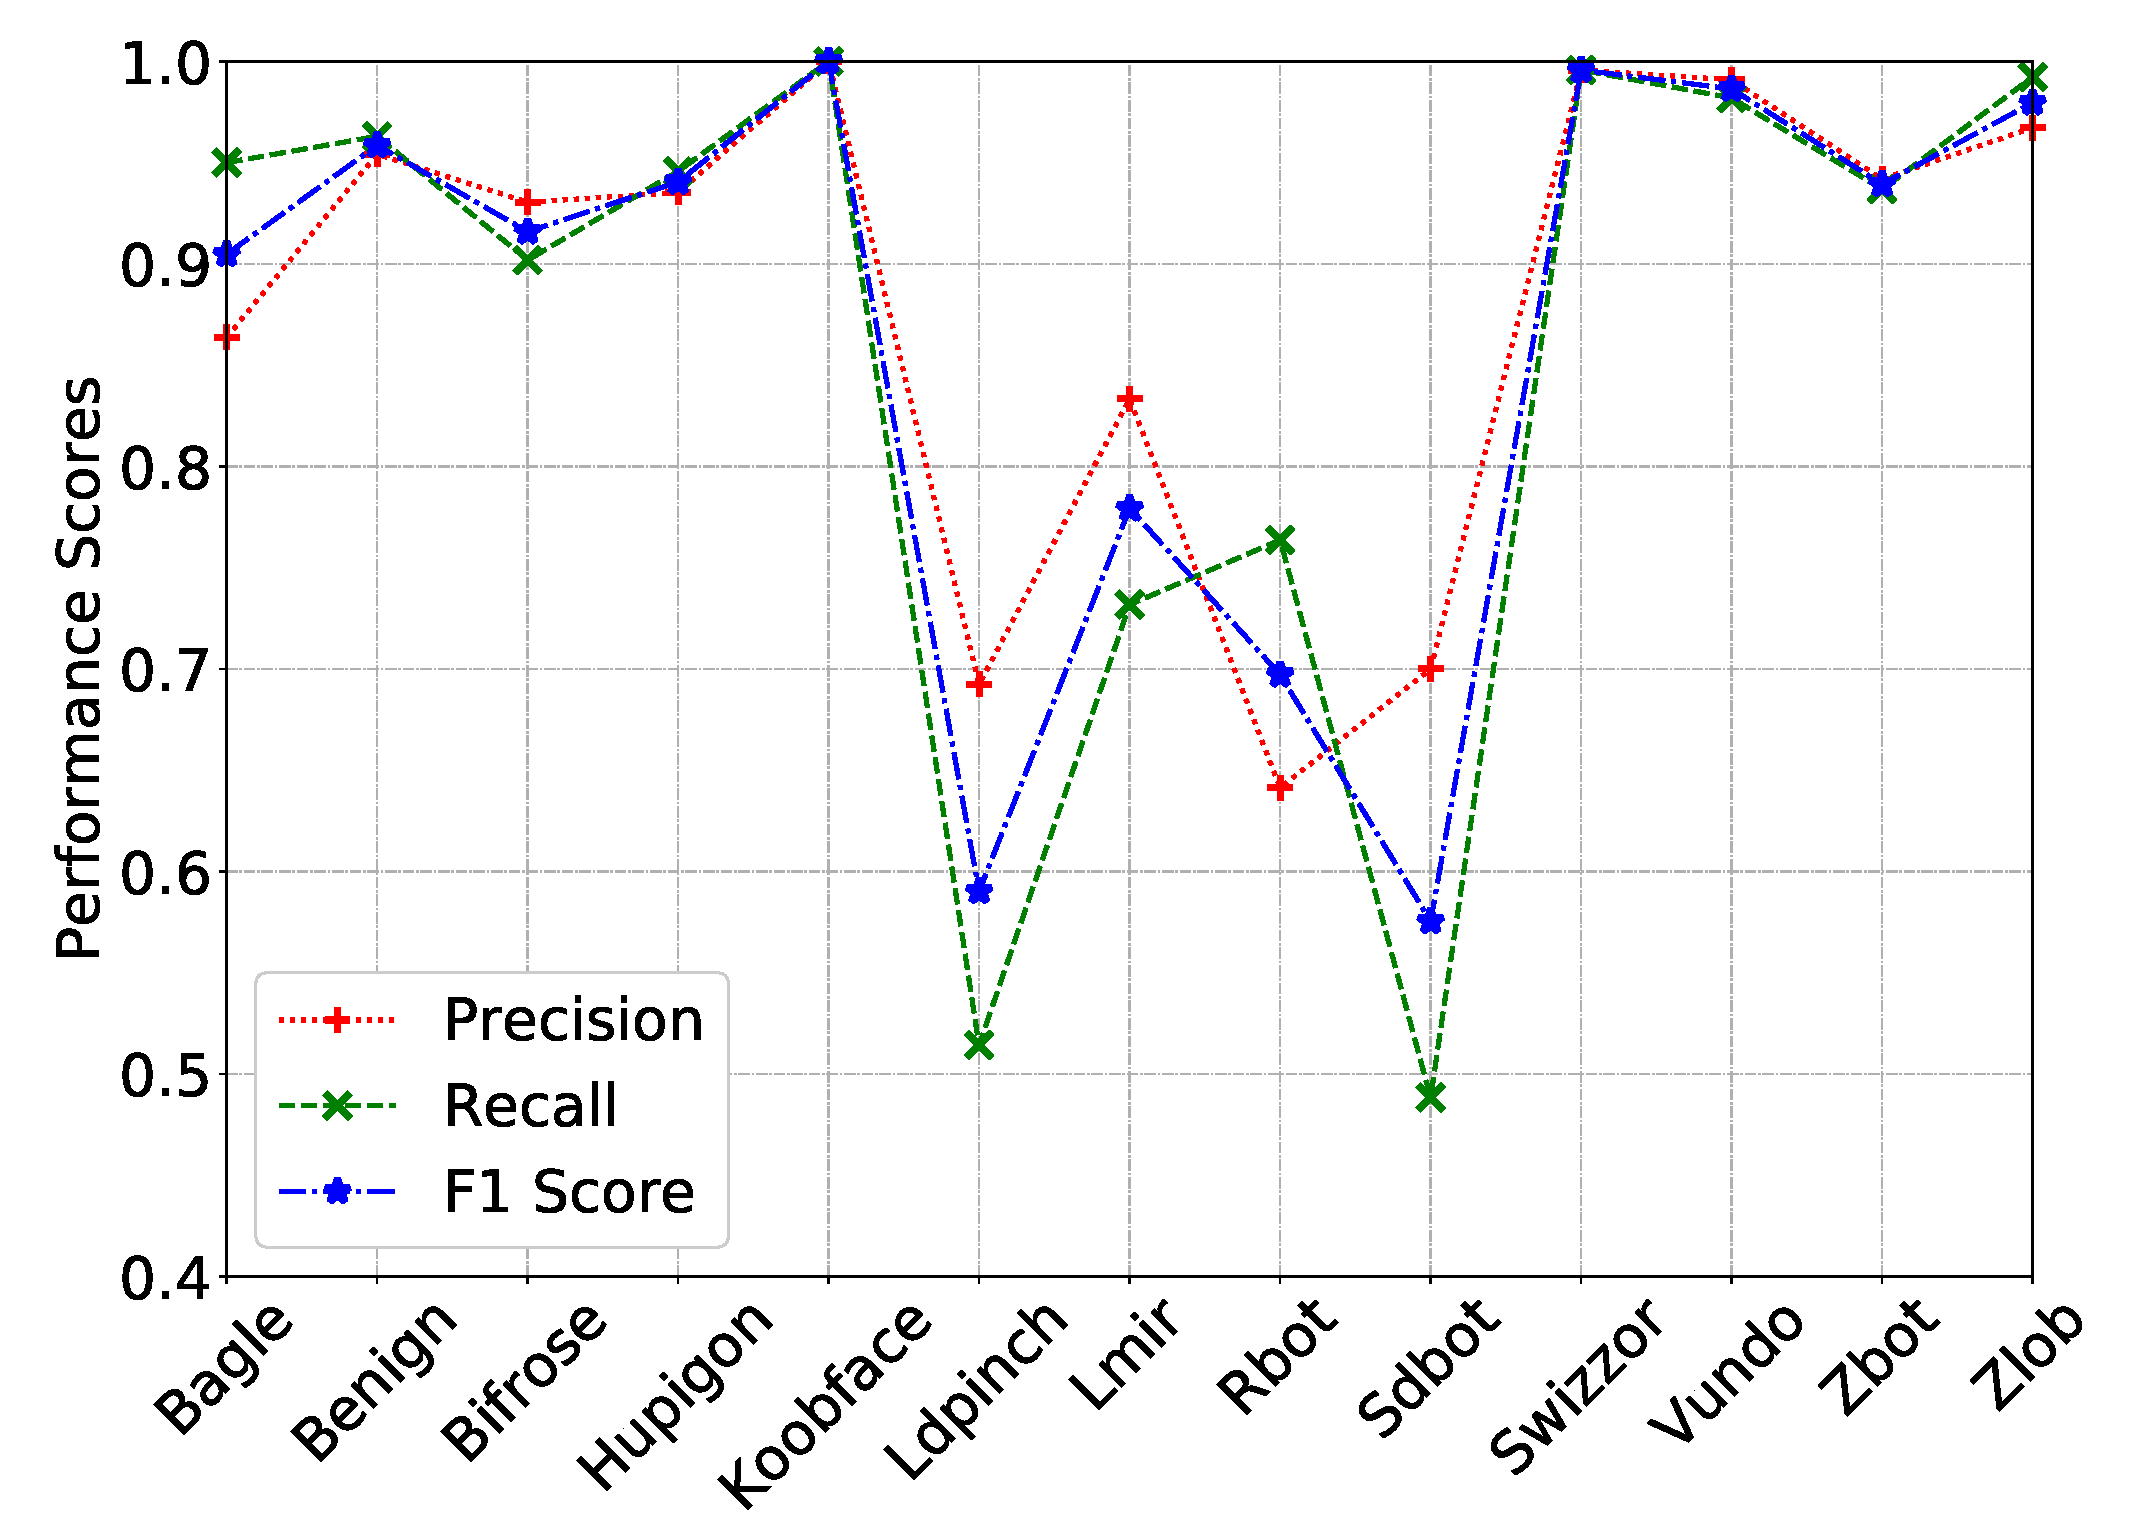
\includegraphics[width=0.90\textwidth]{Magic/figures/YanAcfgScores.eps}}
    \caption{Cross-Validation Scores of \sysname on the YANCFG Dataset.}
    \label{MG:Fig:YANCFGScores}
\end{figure}

\begin{figure}
    \centerline{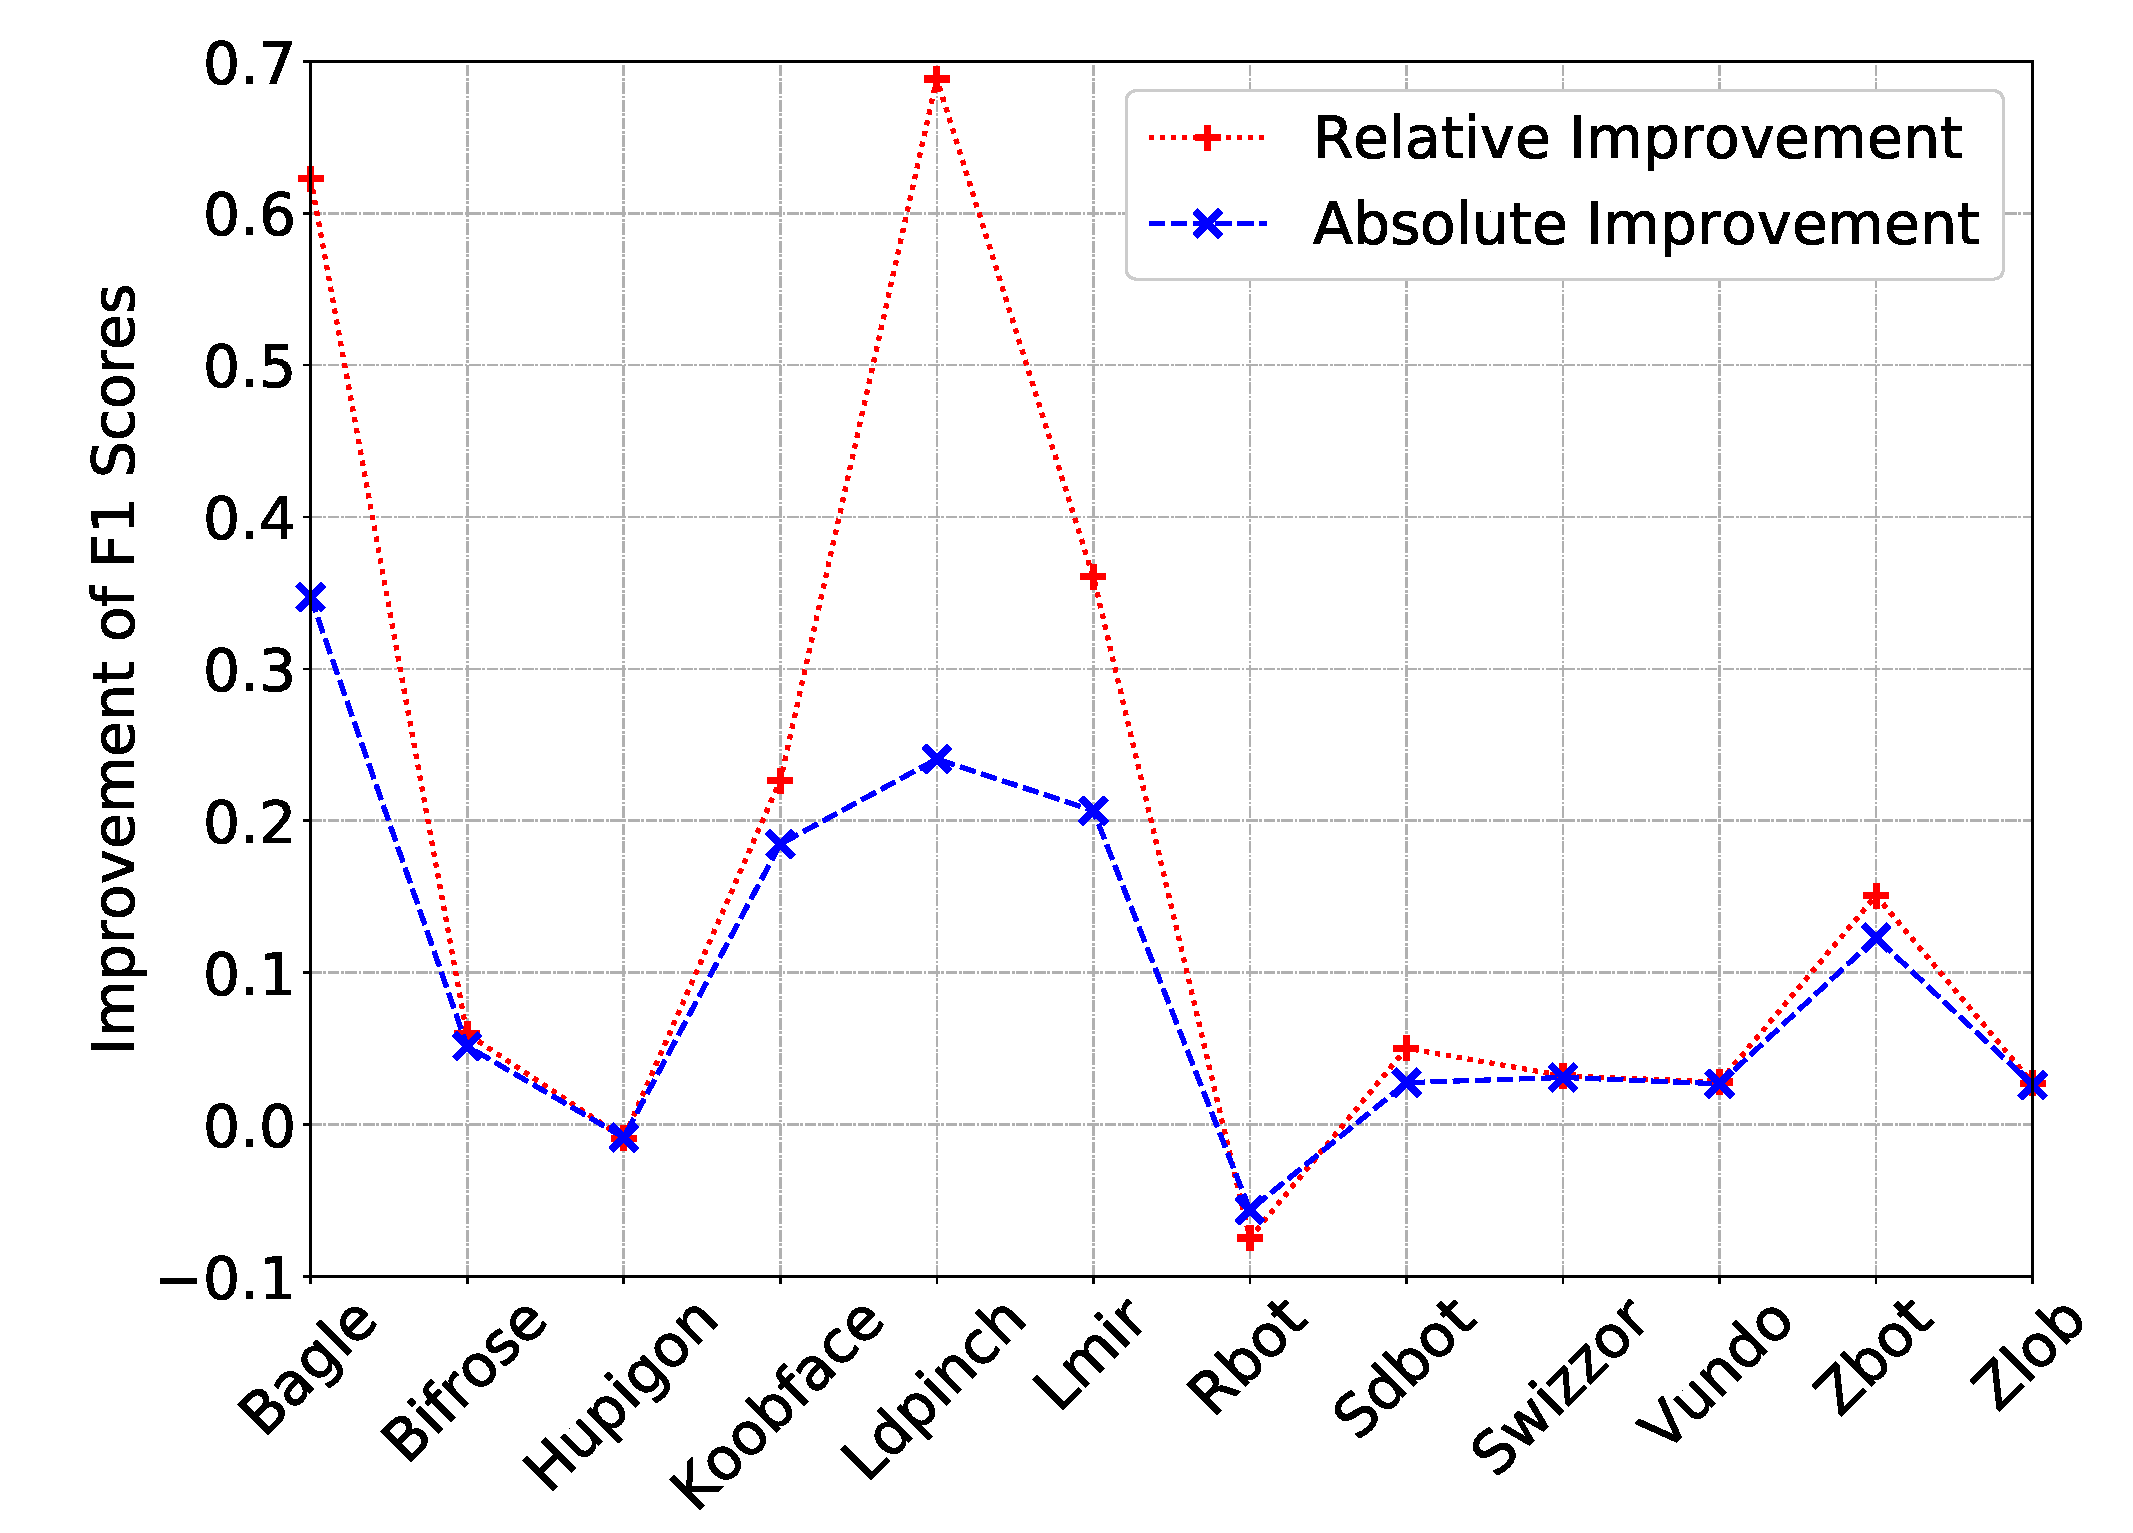
\includegraphics[width=0.90\textwidth]{Magic/figures/YanAcfgF1Improve.eps}}
    \caption{F1 Score Comparison between \sysname and ESVC\cite{YanDataset} on the YANCFG Dataset.
    Improvement on the classification accuracy of benign samples is not shown because it is not reported in \cite{YanDataset}.}
    \label{MG:Fig:YANCFGF1Improve}
\end{figure}

% \begin{table*}
% \centering
% \caption{Confusion Matrix on the YANCFG Dataset}
% \begin{tabular}{l|rrrrrrrrrrrrr}
%   Family &  Bagle &  Benign &  Bifrose &  Hupigon &  Koobface &  Ldpinch &  Lmir &  Rbot &  Sdbot &  Swizzor &  Vundo &  Zbot &  Zlob \\
% \hline
% \hline
%     Bagle &     19 &       0 &        0 &        0 &         0 &        0 &     0 &     1 &      0 &        0 &      0 &     0 &     0 \\
%    Benign &      0 &     104 &        1 &        1 &         0 &        0 &     0 &     0 &      0 &        1 &      0 &     0 &     1 \\
%   Bifrose &      0 &       2 &      294 &       14 &         0 &        3 &     2 &     8 &      1 &        0 &      1 &     0 &     1 \\
%   Hupigon &      1 &       0 &        8 &      766 &         0 &        0 &     3 &    18 &      6 &        0 &      3 &     5 &     0 \\
%  Koobface &      0 &       0 &        0 &        0 &        20 &        0 &     0 &     0 &      0 &        0 &      0 &     0 &     0 \\
%   Ldpinch &      2 &       0 &        2 &        6 &         0 &       18 &     0 &     4 &      0 &        0 &      0 &     3 &     0 \\
%      Lmir &      0 &       2 &        0 &        7 &         0 &        1 &    30 &     1 &      0 &        0 &      0 &     0 &     0 \\
%      Rbot &      0 &       0 &        5 &       16 &         0 &        0 &     1 &    84 &      2 &        0 &      0 &     1 &     1 \\
%     Sdbot &      0 &       1 &        2 &        4 &         0 &        2 &     0 &    12 &     21 &        0 &      0 &     1 &     0 \\
%   Swizzor &      0 &       0 &        0 &        1 &         0 &        0 &     0 &     0 &      0 &      232 &      0 &     0 &     0 \\
%     Vundo &      0 &       0 &        3 &        1 &         0 &        0 &     0 &     1 &      0 &        0 &    542 &     0 &     5 \\
%      Zbot &      0 &       0 &        1 &        3 &         0 &        1 &     0 &     1 &      0 &        0 &      1 &   178 &     5 \\
%      Zlob &      0 &       0 &        0 &        0 &         0 &        1 &     0 &     1 &      0 &        0 &      0 &     1 &   384 \\
% \end{tabular}
% \label{MG:Tab:YANCFGConfusionMatrix}
% \end{table*}

